\documentclass[sigconf,review]{acmart}

%% EDBT 2027 template: A4 geometry and the EDBT macros.
\geometry{twoside=true, head=13pt,
     a4paper,
     includeheadfoot, columnsep=2pc,
     top=57pt, bottom=73pt, inner=54pt, outer=54pt,
     marginparwidth=2pc,heightrounded
     }%
\AtBeginMaketitle{%
  %% EDBT Conference Proceedings setup for ACM sigconf Style



%% EDBT: ISBN and year have to be adapted with every Number / Volume !
%%
\def\EDBTISSN{xxxx-xxxx}
\def\EDBTISBN{xxx-x-xxxxx-xxx-x}
\setcopyright{none}
\copyrightyear{\copyright\ 2027 Copyright held by the owner/author(s).
  Published on xxxxx under ISBN \EDBTISBN, series ISSN \EDBTISSN.
  Distribution of this paper is permitted under the terms of the
  Creative Commons license CC-by-nc-nd 4.0}
\acmYear{2027}
\acmDOI{}
\acmISBN{}


%% These commands are for a PROCEEDINGS abstract or paper.
%% EDBT: This needs adaptation every year!
\acmConference[EDBT '27]{Extending Database Technology}{6-9 April 2027}{Lille (France)}
%%
%%  Uncomment \acmBooktitle if the title of the proceedings is different
%%  from ``Proceedings of ...''!
%%
%%\acmBooktitle{Woodstock '18: ACM Symposium on Neural Gaze Detection,
%%  June 03--05, 2018, Woodstock, NY}


%% EDBT:
\settopmatter{printacmref=false, printccs=false, printfolios=false}


%% EDBT:
%% Macro to make image usable as hyperlink [see http://tex.stackexchange.com/questions/31819/xelatex-includegraphics-and-hyperlink]
\newsavebox{\ximagebox}
\newlength{\ximageheight}
\newsavebox{\xglyphbox}
\newlength{\xglyphheight}
\newcommand{\xbox}[1]%
  {\savebox{\ximagebox}{#1}%
  \settoheight{\ximageheight}{\usebox{\ximagebox}}%
  \savebox{\xglyphbox}{\color{white}\char32}%
  \settoheight{\xglyphheight}{\usebox{\xglyphbox}}%
  \raisebox{\ximageheight}[0pt][0pt]{\raisebox{-\xglyphheight}[0pt][0pt]{%
    \makebox[0pt][l]{\usebox{\xglyphbox}}}}%
    \usebox{\ximagebox}%
    \raisebox{0pt}[0pt][0pt]{\makebox[0pt][r]{\usebox{\xglyphbox}}}}

%% now use this to define the logo header:

\newsavebox{\LogoBox}
\sbox{\LogoBox}{}

%% now define our header and footer for the first page
\fancypagestyle{firstpagestyle}{%
  \fancyhf{}%
  \fancyfoot{}%
  \fancyhead[L,C]{}
  \fancyhead[R]{}{\raisebox{15pt}[0pt][0pt]{\xbox{\usebox{\LogoBox}}}}
  }

\hypersetup{%
  pdfcopyright={CC-by-nc-nd},
  pdfcreator={LaTeX with acmart, hyperref, and EDBT modifications},
  pdfvolumenum={XX},
  pdfissuenum={X},
  pdfisbn={\EDBTISBN},
  pdfissn={\EDBTISSN}
}

}

\usepackage{booktabs}
\usepackage{graphicx}
\usepackage{amsmath}

\newcommand{\inputif}[1]{\IfFileExists{#1}{\input{#1}}{}}
\inputif{../results/paper/final/numbers.tex}
\inputif{../results/paper/final/operators.tex}
\inputif{../results/paper/final/sources.tex}
\inputif{../results/paper/final/streams.tex}
\inputif{../results/paper/final/single_run.tex}
\graphicspath{{../results/paper/final/}}

\begin{document}

\title{[Short Paper] One Query per Template: Moving Query Runtime Models to New Hardware}

\author{Krish Patel}
\email{kmp.patel@uwaterloo.ca}
\orcid{0009-0006-3064-0086}
\affiliation{%
  \institution{University of Waterloo}
  \city{Waterloo}
  \country{Canada}}

\renewcommand{\shortauthors}{Krish Patel}

\begin{abstract}
A model that predicts query runtimes is trained on measurements from one
machine. When the database moves to other hardware, its plans stay the
same but their runtimes change. We ask how to adapt such a model from $k$
queries measured on the new machine. On PostgreSQL we measured 1,162 TPC-H
and TPC-DS queries in six environments that run identical plans: a laptop
and a server, each with all processors and with PostgreSQL pinned to one
processor, the server also pinned to two, and the laptop with a small
buffer pool. The slowdown between two environments is far from a single
factor: most of its variance lies between query templates, and for changes
of processor count or hardware, whether a plan runs in parallel and how
long it runs explain much of it. A single speed factor therefore stops
improving after a few queries. Our correction recalibrates serial and
parallel plans with separate lines and adds an offset for every measured
template. With one measured query per template it brings the moved model's
median Q-error, averaged over templates, to
\PLadTpchLowdimTemplateRoundRobin{} on TPC-H and
\PLadTpcdsLowdimTemplateRoundRobin{} on TPC-DS, close to what it gives a
model trained on the new machine (\PLadTpchLowdimTemplateControlRoundRobin{}
and \PLadTpcdsLowdimTemplateControlRoundRobin): once every template has a
query, the move itself costs little, and the separate lines matter mainly
before that point, more on TPC-H than on TPC-DS. On templates never
measured, no correction does much better than the speed factor, whose error
is close to that of retraining. We fixed five hypotheses before the labels
of \PHPairs{} pairs existed; all five hold as registered, though one falls
short when counted by confidence intervals.
\end{abstract}

\keywords{query performance prediction, learned cost models, hardware change, model adaptation, PostgreSQL}

\maketitle

\section{Introduction}
\label{sec:intro}
Predicting how long a query will run before it runs serves admission
control, scheduling, provisioning and the choice between plans. Learned
models predict runtimes from plan features far better than raw optimizer
costs when they are trained on the system they predict
\cite{ganapathi2009,akdere2012,marcus2019,sun2020}. A runtime, however, is
a property of a plan on a machine, and machines change: a database moves to
new hardware, to a cloud instance of another size, or into a container
with fewer processors. The plans stay, and every runtime the model learned
from is now off, by an amount that depends on the query.

Systems answer this in three ways. Some retrain on the new machine: T3
reruns its whole benchmark \cite{rieger2025t3}, and QCFE reruns simplified
queries to refit its per-operator coefficients and then retrains on 200
labeled queries \cite{yan2024qcfe}. Some map every old prediction through
one fitted line, the model shift used to move performance models of
configurable software \cite{valov2017,jamshidi2017}, whose simplest form
rescales every prediction by one speed factor. Others describe the machine
with features and train one model over many machines, as Redshift's Stage
predictor does with the instance type \cite{wu2024stage}. This paper asks
what lies between retraining and rescaling: if we can afford to run $k$
queries on the new machine, which queries should they be, how should their
runtimes be used, and how large must $k$ be?

We study the question with the plans held fixed. We measured 1,162 queries
from 115 templates of TPC-H and TPC-DS on PostgreSQL in six environments
that run identical plans on copies of the same database. Their 30 ordered
pairs, each measured on both workloads, change the processor count, the
hardware, both, the buffer pool, or several of these at once. We
contribute:
\begin{itemize}
\item A measurement of how runtimes shift when only the environment changes
  (Section~\ref{sec:shift}). The slowdown differs widely between templates.
  Whether a plan has parallel workers carries much of a change of processor
  count, and how long the query runs carries much of the move from laptop
  to server; per-operator timings point to the mechanisms.
\item A comparison of corrections, baselines and query selections for 5
  to 200 measured queries (Sections~\ref{sec:adapt} and \ref{sec:select}).
  One measured query per template with a per-template offset brings the
  moved model close to the same correction on a model trained on the new
  machine; refitting the model on the measured queries is far worse at
  these budgets.
\item A negative result for new templates (Section~\ref{sec:unseen}): no
  correction does much better than the speed factor, whose error is close
  to that of retraining, so the remaining error is the model's error on a
  new template, and the move adds little to it.
\item A confirmatory test (Section~\ref{sec:confirm}): we committed five
  hypotheses and the primary method to our repository before any label of
  \PHPairs{} of the pairs existed, and all five hold under the rules we
  fixed.
\end{itemize}

\section{Problem and Methods}
\label{sec:methods}

\textbf{Setting.} A model $f_A$ predicts the log runtime of a query from
features $x$ of its PostgreSQL plan before the query runs, and was trained
on the runtimes of a pool of queries measured on machine $A$. The database
moves to machine $B$ with the same data, statistics and planner settings, so
the planner chooses the same plans; we call $y_B/y_A$ a query's slowdown.
Before $f_A$ is used on $B$ we may run $k$ queries there. Every query
belongs to a template, the parameterized SQL it was generated from; in a
production system templates can be read from query fingerprints such as
PostgreSQL's query identifier.

\textbf{Features and source model.} The 19 plan features are the root's
startup and total cost, estimated rows and width; the number of nodes and
the depth; the largest row estimate of any node and the sum of the nodes'
log row estimates; the counts of all scans, sequential scans, index scans
(bitmap scans included), nested-loop, hash and merge joins, sorts,
aggregates and materializations; the workers planned over all Gather nodes;
and the number of subplans. Costs, rows and widths enter as $\log(1+x)$.
The source model fits a line in $\log(1+\text{total cost})$ to the log
runtime (the cost line) and a random forest to its residuals (300 trees,
at least two queries per leaf, 4 of the 19 features tried at each split)
\cite{breiman2001,pedregosa2011}. Section~\ref{sec:sources} reports four
other source models.

\textbf{Corrections.} All corrections act on the log errors of the $k$
measured queries, $e_i = \log y_i - f_A(x_i)$, and predict
$\log \hat y = f_A(x) + c(x)$ on $B$; fitting a learner to the residuals
of a base model follows \cite{didona2015}.
\begin{itemize}
\item \emph{Speed factor:} $c$ is the mean of the $e_i$.
\item \emph{Affine+parallel:} $c(x) = a + b\,f_A(x) + \pi(x)\,(a' + b'\,f_A(x))$,
  where $\pi(x)$ is 1 for plans with parallel workers; $b$ makes the
  slowdown depend on the predicted runtime. The intercept $a'$ enters only
  when both kinds of plan are among the $k$ queries, the slope $b'$ only
  when each kind has two. The fit is ridge regression \cite{hoerl1970}
  with an unpenalized intercept, its penalty chosen by leave-one-out
  \cite{golub1979} from 45 values between $10^{-6}$ and $10^{5}$, so a large
  penalty gives back the speed factor.
\item \emph{Ridge correction:} ridge regression of $e$ on the 19
  standardized features, fitted the same way.
\item \emph{Template offsets:} the speed factor plus, for every template
  among the $k$ queries, the mean residual of its queries from that factor;
  other templates get the factor alone.
\item \emph{Low-dim + template}, our primary method: affine+parallel plus,
  for every template among the $k$ queries, the mean residual of its
  queries from that line; other templates get the line alone.
\item \emph{1-NN:} the error of the nearest of the $k$ queries in the
  standardized feature space. It needs no template labels.
\end{itemize}
We also compare against two refits, a nonlinear correction and a lookup:
\emph{target only} refits the source pipeline on the $k$ queries alone;
\emph{pooled} refits it on the source pool and the $k$ queries with the
machine as a feature; \emph{forest on the errors} fits a forest to the
$e_i$; and a \emph{template lookup} predicts a query by the mean measured
log runtime of its template, with no model. The \emph{oracle} refits the
source pipeline on the whole target pool. It is a reference, not a bound:
it knows nothing of templates. The \emph{no-move control} applies a method
to a model trained on the target pool itself, with the same $k$ queries;
the gap to it is the cost of the move.

\textbf{Choosing the $k$ queries.} \emph{Random} takes them in a random
order. \emph{Round robin} takes one query of each template in turn, in a
random order of templates and of queries; \emph{cheapest per template} is
round robin with the query that ran fastest on $A$ first. \emph{k-center}
adds the query farthest from those chosen so far in the standardized
feature space \cite{gonzalez1985,sener2018}. \emph{D-optimal} adds the
query that most increases $\det(I + X^\top X)$, where $X$ holds the chosen
queries' standardized features and a column of ones
\cite{wynn1970,mitchell1974}. \emph{Plan class} alternates between parallel
and serial plans. Every strategy derives its $r$-th sequence from the
$r$-th of 20 random orders, so comparisons are paired; none looks at a
runtime on $B$.

\section{Experimental Setup}
\label{sec:setup}

% The wide floats are placed here and in Section 4.1, a page before the text that discusses them,
% so that each lands at the top of the page where its discussion starts.
\begin{table*}[t]
\caption{How the runtime of the same plan changes, for seven of the 30 ordered pairs of each workload. Slowdown: median of target over source runtime, for serial plans and plans with parallel workers. Template share: the share of the variance of the log slowdown between templates (shift), the same corrected for the number of templates ($\epsilon^2$), and the share between two passes on the source alone (noise). $R^2$: least-squares fits of the log slowdown on whether the plan is parallel, on the log source runtime (size) and on both with their interaction; features (new): a ridge model on the 19 features scored on templates (TPC-DS: families) left out of its fit, which can be negative.}
\label{tab:shift}
\small
\inputif{../results/paper/final/table_shift_paper.tex}
\end{table*}

\textbf{Environments.} M1 is a laptop (Intel Core Ultra 7 155H, 22
threads) running PostgreSQL 18.6 in WSL2 (a Linux virtual machine on
Windows) with 16\,GB of memory; M3 is a virtual machine with 64 virtual
processors of an AMD EPYC 9754 and 1\,TB of memory on a shared university
server. M2 and M4 are M1 and M3 with every
PostgreSQL server process pinned to one virtual processor, so that a plan's
leader and its parallel workers (at most two per Gather node) share it
while the client keeps all processors; M6 is M3 pinned to two. M5 is M1
with PostgreSQL's default buffer pool, 128\,MB instead of 2\,GB. All use
the same PostgreSQL build, which has no JIT, and the same settings
(work\_mem 64\,MB, effective\_cache\_size 8\,GB) apart from M5's buffer
pool, on copies of the same database files; every saved plan, with its
estimates and costs, is identical in all six. The data fit in memory
everywhere.

\textbf{Workloads.} TPC-H at scale factor 1 \cite{tpch}: 680 queries from
22 templates, 420 from its query generator and 260 with range parameters
drawn wider than the specification's, so that runtimes vary inside a
template. TPC-DS at scale factor 1 \cite{tpcds}: 482 queries from the 93
templates whose first query ran within 30\,s on M1; in its four templates
of two statements, each statement counts as a query of the template.
Queries are split once, inside every template, into a pool from which the
$k$ queries are drawn (476 and 294 queries, 70\% and 61\%) and a test set
on which the corrections are scored. We link two TPC-DS templates when their first
queries, with literals masked, share at least 85\% of their tokens, and take
the connected components as families: 75 families, 15 of them with more
than one template.

\textbf{Labels.} Every environment runs every query in three passes in
different random orders; in a pass a query runs four times with
\texttt{EXPLAIN (ANALYZE, TIMING OFF)}, the first only to warm the cache.
A run's time is the execution time PostgreSQL reports, without planning or
sending rows to the client, and a label is the median over passes of the
median of the three timed runs. A pass whose level shifts by more than 10\%
partway through, or during which the laptop slept or ran on battery, is
measured once more. The median Q-error between two passes of the same
query is \NoiseMedQMin{} to \NoiseMedQMax{} per environment and workload.
For Section~\ref{sec:shift} we also ran every query once more in M1 to M5
with per-node timing on, after a warm-up; an operator's own time is its
time over all loops minus its children's, and these timings are never
labels.

\textbf{Measures.} The error of a test template is the median Q-error
($\max(\hat y/y, y/\hat y)$) of its test queries; a method's error is the
geometric mean of the template errors, averaged in log over 20 random
orders of the pool (5 in the test on new templates). Ratios between two
methods are geometric means over templates of the ratio of their errors,
with 95\% intervals from 2000 resamples of templates (of families in
TPC-DS), paired across methods; one method \emph{beats} another when that
interval lies below 1. The test on new templates holds out one template at
a time (in TPC-DS its family): the source model is retrained on $A$'s pool
without it, the $k=25$ queries are drawn from $B$'s pool without it, the
oracle is retrained on that pool, and the template's test queries are
scored.

\textbf{Exploratory and confirmatory analyses.} We designed the
corrections and strategies on TPC-H with M1, M2 and M3, so those pairs are
exploratory. We committed the primary method (low-dim + template with
round-robin selection) and five hypotheses (commit 17c328f) after the
first TPC-DS passes on M2 and M3 had started and before any label of TPC-DS
on M2, M3 or M4 or of TPC-H on M4 existed; Section~\ref{sec:confirm} tests
them on the \PHPairs{} pairs these labels form. Within twenty minutes, still
before any such label existed, a code review led to an amendment (commits
b2e59dc and fc9dc9a): TPC-DS intervals resample families, the test on new
templates holds out families, and affine+parallel and the primary method
leave out their parallel terms when the $k$ queries hold one plan class.
The per-operator timings and the results of Section~\ref{sec:sources} are
exploratory, as are M5, M6, the no-move control, the lookup and the
single-run labels of Section~\ref{sec:select}, which were added later.

\section{Results}
\label{sec:results}

\subsection{How runtimes shift}
\label{sec:shift}

Table~\ref{tab:shift} shows seven pairs per workload. No single factor
describes any of them. Over all pairs, a share of \PSRTpchShareMin{} to
\PSRTpcdsShareMax{} of the variance of the log slowdown lies between
templates (\PSRTpchEpsilonTwoMin{} to \PSRTpcdsEpsilonTwoMax{} after
correcting for the number of templates), against at most
\PSRTpchNoiseMax{} (TPC-H) and \PSRTpcdsNoiseMax{} (TPC-DS) between two
passes of one machine. What separates the templates depends on the change.
Pinning PostgreSQL to one processor roughly doubles the runtime of plans
with parallel workers and leaves serial plans almost unchanged, and that one
bit explains about half of the variance; with two processors (M3$\to$M6)
parallel plans slow by only \PSTpchMThreetoMSixParallelX{} (TPC-H) and
\PSTpcdsMThreetoMSixParallelX{} (TPC-DS). Moving from the laptop to the server slows serial and
parallel plans alike, but short queries more than long ones: the log
slowdown falls as the log runtime grows, and size explains
\PSTpchMOnetoMThreeRTwoSize{} (TPC-H) and \PSTpcdsMOnetoMThreeRTwoSize{}
(TPC-DS) of it. The small buffer pool moves the median runtime by a factor
of only \PSTpchMOnetoMFiveSlowdown{} (TPC-H) and
\PSTpcdsMOnetoMFiveSlowdown{} (TPC-DS), although TPC-H's serial plans slow
by \PSTpchMOnetoMFiveSerial, and no coarse plan property explains it.

\begin{table}[t]
\caption{Median ratio of each operator's own time (target over source), inside (par.) and outside (ser.) the parallel part of plans, over the nodes of both workloads weighted by the source's time, from one extra pass with per-node timing. Proc.: one processor (M1$\to$M2, M3$\to$M4); hardware: M1$\to$M3; buffer pool: M1$\to$M5.}
\label{tab:ops}
\footnotesize
\setlength{\tabcolsep}{2.4pt}
\inputif{../results/paper/final/table_operators.tex}
\end{table}

\begin{figure*}[t]
\centering
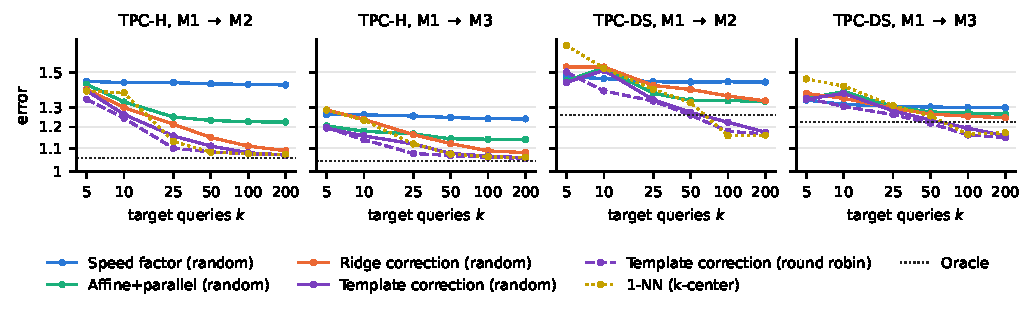
\includegraphics[width=\textwidth]{fig_learning_main}
\Description{Four line charts of the error against the number of measured queries for five corrections and the oracle; the speed factor stays flat and the primary method with round-robin selection falls to the oracle on TPC-H and below it on TPC-DS.}
\caption{Error (geometric mean over test templates of the median Q-error) against the number $k$ of measured target queries, both axes logarithmic, for a processor change (M1$\to$M2) and a hardware change (M1$\to$M3) on each workload; the TPC-H panels are pairs the methods were designed on. Line style gives the selection: solid random, dashed round robin, dotted k-center. The horizontal dotted line is the oracle.}
\label{fig:learning}
\end{figure*}

\begin{table*}[t]
\caption{Error by kind of change, as the geometric mean over its ordered pairs. Speed, Aff.+par.\ and Ridge use random selection; Primary (low-dim + template) uses random selection at $k=10$ and round robin at $k=25$ and $k=100$. Oracle: the source pipeline refitted on the whole target pool. New templates: each template (TPC-DS: its family) held out from the source model, the $k=25$ randomly chosen queries, the oracle and every correction. Mixed: the remaining 14 pairs, all involving M5 or M6.}
\label{tab:adapt}
\small
\setlength{\tabcolsep}{4.6pt}
\inputif{../results/paper/final/table_adapt_paper.tex}
\end{table*}

Per-operator timings point to the mechanisms (Table~\ref{tab:ops}),
although per-node timing adds overhead that differs between machines. On
one processor, the main operators of each workload (at least 3\% of its
time on the source; Table~\ref{tab:ops} pools the workloads and also lists
smaller ones) take \OpProcParallel{} times as long inside the parallel part
of a plan on the laptop and \OpServerProcParallel{} times on the server,
while serial operators keep their speed: the same mechanism on both
machines. The move from laptop to server slows operators
unevenly, by \OpHwRange{} times depending on the operator, so plans with
different operators slow differently. With the small buffer pool, index
scans, which revisit pages that no longer stay in PostgreSQL's buffers,
slow down \OpMemIndex{} times, while sequential scans, which read pages in
order, change by \OpMemSeq. Which templates slow down thus depends on their
operators, which plan-level features see only in part: a ridge model on the
19 features, fitted without the template it predicts, explains at most
\PSRTpchRTwoLotMax{} of the variance, and nothing for the buffer pool (last
column of Table~\ref{tab:shift}).

\subsection{Adapting with $k$ queries}
\label{sec:adapt}

\begin{table}[t]
\caption{Error at the budget where each template can have one query, as the geometric mean over the 30 ordered pairs of a workload; the last row applies the primary method to a model trained on the target itself (no move).}
\label{tab:ladder}
\small
\setlength{\tabcolsep}{3pt}
\inputif{../results/paper/final/table_ladder.tex}
\end{table}

Figure~\ref{fig:learning} and Table~\ref{tab:adapt} give the errors, and
Table~\ref{tab:ladder} compares the methods at one query per template.
Without adaptation the source model errs by \PNoneTpchKTwoFive{} on TPC-H
and \PNoneTpcdsKOneZeroZero{} on TPC-DS. The speed factor finds the
average slowdown from a few queries and then stays flat (TPC-H:
\PSpeedTpchKFive{} at $k=5$, \PSpeedTpchKTwoFive{} at $k=25$; TPC-DS:
\PSpeedTpcdsKFive{} and \PSpeedTpcdsKTwoFive), because no single factor
fits templates whose slowdowns differ. Affine+parallel helps at small
budgets on TPC-H: it beats the speed factor at $k=10$ in \PAffTPCHBelow{}
of \PAffTPCHPairs{} pairs and loses in \PAffTPCHAbove; for processor
changes it lowers the $k=10$ error from \PATpchProcessorsRandomSpeedOneZero{}
to \PATpchProcessorsRandomAffineParallelOneZero, and the primary method's
template offsets bring it to \PATpchProcessorsRandomLowdimTemplateOneZero.
On TPC-DS, affine+parallel beats the speed factor at $k=10$ in
\PAffTPCDSBelow{} pairs and loses in \PAffTPCDSAbove, and its lead grows
with $k$ (Figure~\ref{fig:learning}).

Once each template has a measured query, the template offsets carry the
gain. With round-robin selection the primary method reaches
\PLadTpchLowdimTemplateRoundRobin{} on TPC-H at $k=25$ and
\PLadTpcdsLowdimTemplateRoundRobin{} on TPC-DS at $k=100$; offsets on the
speed factor alone give \PLadTpchTemplateRawRoundRobin{} and
\PLadTpcdsTemplateRawRoundRobin, so the affine+parallel line lowers the
error by about 1\% on TPC-H and by almost nothing on TPC-DS. The same
correction on a model trained on the target itself reaches
\PLadTpchLowdimTemplateControlRoundRobin{} and
\PLadTpcdsLowdimTemplateControlRoundRobin: the move costs little. Without
the correction, that model is the oracle, which refits the template-blind
pipeline on the whole target pool. On TPC-H the oracle errs by only
\PLadTpchOracleRandom, so there the correction itself costs about 3\%; on
TPC-DS it reaches only \PLadTpcdsOracleRandom, since three pool queries
per template are too few for its forest, and the primary method is
\PPrimOracleTPCDSMin{} to \PPrimOracleTPCDSMax{} times the oracle's error
in every pair. The model matters inside a template: a lookup of the
measured runtime per template errs by \PLadTpchLookupRoundRobin{} on TPC-H
against \PLadTpchLowdimTemplateRoundRobin{} for the primary method, because
the widened queries vary inside their templates; on TPC-DS, whose queries
vary inside a template by a factor of only \PSpreadTPCDS{} (median
geometric standard deviation), the gap is smaller
(\PLadTpcdsLookupRoundRobin{} against \PLadTpcdsLowdimTemplateRoundRobin).
The refits and the forest on the errors ran with random selection only.
With the same selection the primary method reaches
\PLTpchKTwoFiveRandomLowdimTemplate{} and
\PLTpcdsKOneZeroZeroRandomLowdimTemplate{} (Table~\ref{tab:select}),
against \PLadTpchTargetRandom{} and \PLadTpcdsTargetRandom{} for target
only, \PLadTpchPooledRandom{} and \PLadTpcdsPooledRandom{} for the pooled
refit, and \PLadTpchForestResidRandom{} and \PLadTpcdsForestResidRandom{}
for a forest on the errors.

\subsection{Which queries to measure}
\label{sec:select}

\begin{table}[t]
\caption{Error of three corrections (columns) when the $k$ queries are chosen by each strategy (rows), as the geometric mean over the 30 ordered pairs of a workload, at the smallest budget of our grid that holds one query per template. Seconds: total runtime of the $k$ queries on the target, one run each.}
\label{tab:select}
\small
\inputif{../results/paper/final/table_selection_paper.tex}
\end{table}

Table~\ref{tab:select} compares the strategies. Covering the templates is
what matters. On TPC-H at $k=25$, round robin lowers the primary method's
error from \PLTpchKTwoFiveRandomLowdimTemplate{} to
\PLTpchKTwoFiveRoundRobinLowdimTemplate. Without template labels, k-center
selection with the 1-NN correction comes close on TPC-H
(\PLTpchKTwoFiveKCenterOneNn) and matches the primary method on TPC-DS at
$k=100$ (\PLTpcdsKOneZeroZeroKCenterOneNn{} against
\PLTpcdsKOneZeroZeroRoundRobinLowdimTemplate, lower in
\PNnBelowPrimTPCDS{} pairs), since queries of one template have near
plans. D-optimal selection, which is built for the ridge correction, gives
that correction its lowest TPC-DS error, but on TPC-DS it picks long queries
(\PLTpcdsKOneZeroZeroDOptimalCalibrationS\,s against
\PLTpcdsKOneZeroZeroRoundRobinCalibrationS\,s for round robin) and worsens
the primary method; on TPC-H it picks the cheapest set. Measuring the
cheapest query of each template saves about a quarter of the time but
costs accuracy, since short queries shift differently from long ones.
Running the round-robin queries once takes about
\PLTpchKTwoFiveRoundRobinCalibrationS\,s on TPC-H and
\PLTpcdsKOneZeroZeroRoundRobinCalibrationS\,s on TPC-DS, while the
corrections above use labels from three passes. With one run per query
instead, all from one pass as in a single session, the primary method errs
by \SingleTpchWarmLowdimTemplate{} on TPC-H and
\SingleTpcdsWarmLowdimTemplate{} on TPC-DS when that run is warm, and by
\SingleTpchFirstLowdimTemplate{} and \SingleTpcdsFirstLowdimTemplate{} when
it is the query's first run in the pass; the no-move control rises about
as much (to \SingleTpchFirstControl{} and \SingleTpcdsFirstControl), so the
move still costs little.

\subsection{New templates}
\label{sec:unseen}

The last four columns of Table~\ref{tab:adapt} test templates absent from
the $k$ queries and from every model's training. Here no correction does
much better than the speed factor: affine+parallel is within a few percent
of it, and the ridge correction is worse, since its feature slopes, fitted
to the measured templates, do not carry to a new one. Retraining helps
little: the oracle, retrained on the target pool outside the held-out
template, errs by \PARTpchHardRandomOracleMin{} to
\PARTpchHardRandomOracleMax{} on TPC-H and \PARTpcdsHardRandomOracleMin{}
to \PARTpcdsHardRandomOracleMax{} on TPC-DS, about as much as the speed
factor, whose error is at most \PHHFourMaxAll{} times the oracle's in any
pair. These errors are the model's on a template it has never seen, as
plan-level models have long shown \cite{akdere2012}; the move to a new
machine barely adds to them.

\subsection{Other source models and streams}
\label{sec:sources}

The primary method's advantage does not depend on the source model. With
a random forest, gradient-boosted trees, ridge regression or the cost line
as $f_A$, it beats the speed factor at one query per template in all
\SrcWinsTotal{} combinations of source model, workload and pair. It also
repairs weak models: on the cost line alone, whose oracle errs by
\SrcTpchCostOracle{} on TPC-H and \SrcTpcdsCostOracle{} on TPC-DS, it
reaches \SrcTpchCostPrimary{} and \SrcTpcdsCostPrimary. We also replay
each pair's test queries as a stream that runs on the source machine and
then, without warning, on the target, in batches of about ten queries,
each predicted before it is learned from \cite{gama2013}. Over the last
five batches, the primary method refitted on the last 50 queries reaches a
batch median Q-error of \StreamFinalLowdimTemplateLastFiveZero{}, against
\StreamFinalRidgeLastFiveZero{} for the ridge correction on the same
window, \StreamFinalRidgeAll{} for the ridge correction refitted on all
queries seen, whose history keeps the old machine's errors, and
\StreamFinalNever{} without updates.

\subsection{Confirmatory tests}
\label{sec:confirm}

\begin{table}[t]
\caption{The five hypotheses, fixed before any label of the \PHPairs{} confirmatory pairs existed (the 12 ordered TPC-DS pairs among M1 to M4 and the 6 TPC-H pairs with M4), and their results. H2 counts pairs whose 95\% interval lies below 1; H3 and H5 count pairs whose ratio is below 1, as registered; H4 bounds the speed factor's error over the oracle's.}
\label{tab:hyp}
\small
\begin{tabular}{@{}lp{0.66\columnwidth}l@{}}
\toprule
& Hypothesis and result & \\
\midrule
H1 & Template share above 0.5 in every pair (both directions of a pair share one value); smallest \PHHOneMin. & \PHHOnePass \\
H2 & $k=100$: primary (round robin) beats the speed factor (random) in every pair and the ridge correction (random) in at least two thirds; \PHHTwoVsSpeedOk{} and \PHHTwoVsRidgeOk{} of \PHHTwoN. & \PHHTwoPass \\
H3 & $k=10$: affine+parallel (random) has a lower error than the speed factor (random) in at least three quarters of the pairs that change the processor count; \PHHThreeOk{} of \PHHThreeN. & \PHHThreePass \\
H4 & New templates: the speed factor's error is at most 1.15 times the oracle's in every pair; largest \PHHFourMax. & \PHHFourPass \\
H5 & $k=100$: k-center with 1-NN has a lower error than random selection with the ridge correction in at least two thirds; \PHHFiveOk{} of \PHHFiveN. & \PHHFivePass \\
\bottomrule
\end{tabular}
\end{table}

Table~\ref{tab:hyp} lists the hypotheses with their results on the
\PHPairs{} pairs whose labels did not exist when we fixed them. All five
hold under the registered rules. Counted by intervals instead, H5 still
holds (\PHHFiveOkCI{} of \PHHFiveN{} pairs), but H3 has \PHHThreeOkCI{} of
\PHHThreeN, short of its threshold: the small-budget gain of
affine+parallel is real on TPC-H and uncertain on TPC-DS.

\section{Related Work}
\label{sec:related}
\textbf{Learned runtime models and hardware.} Learned models predict query
runtimes from plan features
\cite{ganapathi2009,akdere2012,marcus2019,sun2020,zhao2022}, and most are
trained for one deployment. T3 moves to new hardware by rerunning its
benchmark and retraining \cite{rieger2025t3}; zero-shot cost models
transfer across databases on one machine and leave hardware features to
future work \cite{hilprecht2022}; a recent drift benchmark and an
experimental study cover data and workload drift, not hardware
\cite{zhao2026neurbench,meng2026drift}; and a recent tutorial lists
aligning label collection with the production hardware as open
\cite{heinrich2025tutorial}. Redshift's Stage predictor feeds the instance
type to a global model trained across its fleet and backs it with a model
and a cache of repeated queries for each instance \cite{wu2024stage};
Costream takes hardware features as input for stream processing
\cite{heinrich2024costream}; and Packing Light predicts the throughput of
TPC-H and TPC-DS mixes on new cloud hardware from fingerprints taken on a
few sampled configurations \cite{duggan2013}. The closest work moves a cost
model to a second machine: QCFE refits per-operator coefficients from
queries run there and retrains on 200 labeled queries \cite{yan2024qcfe},
DACE fine-tunes on a whole workload rerun on the second machine
\cite{liang2024dace}, and ParamTree predicts PostgreSQL's cost constants
from a machine's hardware and settings and, on unseen cloud servers, beats
both a linearly scaled cost model and one calibrated on samples from each
server \cite{yang2023}. Older work calibrates cost formulas from measured
queries: Wu et al.\ calibrate PostgreSQL's cost units on each machine with
designed queries \cite{wu2013}, and Zhu and Larson fit a regression cost
formula per query class of a multidatabase system from queries sampled in
that class \cite{zhu1994}, a precursor of our per-template offsets, as is
Cleo's combination of many small cost models for recurring subgraphs with
general ones \cite{siddiqui2020cleo}. We add a controlled measurement of
how much of a hardware shift a handful of queries can absorb, and of which
queries to run.

\textbf{Transferring performance models.} For configurable software, a
fitted line from source to target performance (model shift) carries a
model across hardware when the change is mild
\cite{valov2017,jamshidi2017}, and fails for multithreaded programs or
severe changes \cite{valov2020,jamshidi2017,jamshidi2018}; Libra, which
moves database configuration models across hardware and workloads, finds
that model shift can transfer negatively \cite{nakamori2026libra}. OneProxy
adapts a neural-network latency predictor to a new device from about 50
measurements with one global factor plus sparse per-operator deviations and
aims to preserve rankings \cite{lu2021oneproxy}; our ridge correction has the same form with an L2
penalty. The affine part of our affine+parallel correction is model shift
on the log prediction, and our results show where it stops: a change of
processor count acts through parallel plans, and every change acts through
templates.

\textbf{Model updating and choosing samples.} Clinical prediction research
calls the speed factor \emph{recalibration in the large} and finds that such
simple updates beat revising the whole model unless the new sample is large
\cite{steyerberg2004,vergouwe2017}. Our ridge correction is regularized
least-squares transfer on the source model's residuals, with an
unpenalized intercept and a leave-one-out penalty
\cite{kuzborskij2013}. To choose queries we use greedy D-optimal design
\cite{wynn1970,mitchell1974} and farthest-first selection
\cite{gonzalez1985,sener2018}. Ernest picks the training runs of its linear
runtime model by A-optimal design under a budget on their cost
\cite{venkataraman2016ernest}, which would counter the long queries that
D-optimal selection picks here; L2S uses the source model to choose which
configurations to measure \cite{jamshidi2018}, Warper which queries to use
when it adapts a cardinality estimator \cite{li2022warper}, and Ma et al.\
which queries to label for learned database components
\cite{ma2020active}.

\raggedbottom
\section{Conclusion}
\label{sec:conclusion}
In our study, moving a runtime model to new hardware did not need a new
training set. One measured query per template, with an offset for each
template on the moved model, came close to the same correction on a model
trained on the new machine; separate lines for serial and parallel plans
mattered mostly before every template had a query, and more on TPC-H than
on TPC-DS. For templates never measured, the speed factor was about as
good as anything we tried, because the remaining error is the model's error
on a template it has not seen, and the change of machine adds little to it.
Our study has limits. It covers one database system on two x86 machines,
both virtualized, at scale factor 1, where the data fit in memory in every
environment, and only queries under 30\,s, run warm and one at a time. We
score per-template medians and do not measure tail errors. The 30 pairs of
a workload reuse the labels of six environments, so they are not
independent replications. The processor changes cut a
plan's leader and workers to one or two processors, and pinning keeps the
planner's two workers per Gather; a target with more processors than a
plan's processes would hide most of that effect. Plans are fixed, so a
move that also changes settings or plans is out of scope, and all source
models use the same 19 plan-level features. Operator-level models, other
machines and data larger than memory are the next steps.

\begin{acks}
Claude (Anthropic) was used to generate sections of this work, including
text, tables, graphs, code, data and citations.
\end{acks}

\section*{Artifacts}
{\sloppy The query generators, the measurement and evaluation code, all
labels, plans and per-operator timings, the study plan with its timestamped
amendments, and the scripts that build every number, table and figure of
this paper are at \url{https://github.com/KrishPatel13/query-runtime-transfer}. Its
README lists the commands: \texttt{src/paper\_eval.py} runs the evaluation
from the labels, \texttt{src/paper\_report.py} and its companions write
the tables, figures and \LaTeX{} macros, and \texttt{scripts/} repeats the
measurements.\par}

\balance
\bibliographystyle{ACM-Reference-Format}
\bibliography{../references}

\end{document}
